\documentclass[man,floatsintext]{apa6}
\usepackage{lmodern}
\usepackage{amssymb,amsmath}
\usepackage{ifxetex,ifluatex}
\usepackage{fixltx2e} % provides \textsubscript
\ifnum 0\ifxetex 1\fi\ifluatex 1\fi=0 % if pdftex
  \usepackage[T1]{fontenc}
  \usepackage[utf8]{inputenc}
\else % if luatex or xelatex
  \ifxetex
    \usepackage{mathspec}
  \else
    \usepackage{fontspec}
  \fi
  \defaultfontfeatures{Ligatures=TeX,Scale=MatchLowercase}
\fi
% use upquote if available, for straight quotes in verbatim environments
\IfFileExists{upquote.sty}{\usepackage{upquote}}{}
% use microtype if available
\IfFileExists{microtype.sty}{%
\usepackage{microtype}
\UseMicrotypeSet[protrusion]{basicmath} % disable protrusion for tt fonts
}{}
\usepackage{hyperref}
\hypersetup{unicode=true,
            pdftitle={Speakers of diverse languages structure their utterances for efficient communication},
            pdfauthor={Josef Klafka~\& Daniel Yurovsky},
            pdfkeywords={keywords},
            pdfborder={0 0 0},
            breaklinks=true}
\urlstyle{same}  % don't use monospace font for urls
\usepackage{graphicx,grffile}
\makeatletter
\def\maxwidth{\ifdim\Gin@nat@width>\linewidth\linewidth\else\Gin@nat@width\fi}
\def\maxheight{\ifdim\Gin@nat@height>\textheight\textheight\else\Gin@nat@height\fi}
\makeatother
% Scale images if necessary, so that they will not overflow the page
% margins by default, and it is still possible to overwrite the defaults
% using explicit options in \includegraphics[width, height, ...]{}
\setkeys{Gin}{width=\maxwidth,height=\maxheight,keepaspectratio}
\IfFileExists{parskip.sty}{%
\usepackage{parskip}
}{% else
\setlength{\parindent}{0pt}
\setlength{\parskip}{6pt plus 2pt minus 1pt}
}
\setlength{\emergencystretch}{3em}  % prevent overfull lines
\providecommand{\tightlist}{%
  \setlength{\itemsep}{0pt}\setlength{\parskip}{0pt}}
\setcounter{secnumdepth}{0}
% Redefines (sub)paragraphs to behave more like sections
\ifx\paragraph\undefined\else
\let\oldparagraph\paragraph
\renewcommand{\paragraph}[1]{\oldparagraph{#1}\mbox{}}
\fi
\ifx\subparagraph\undefined\else
\let\oldsubparagraph\subparagraph
\renewcommand{\subparagraph}[1]{\oldsubparagraph{#1}\mbox{}}
\fi

%%% Use protect on footnotes to avoid problems with footnotes in titles
\let\rmarkdownfootnote\footnote%
\def\footnote{\protect\rmarkdownfootnote}


  \title{Speakers of diverse languages structure their utterances for efficient communication}
    \author{Josef Klafka\textsuperscript{1}~\& Daniel Yurovsky\textsuperscript{1,2}}
    \date{}
  
\shorttitle{Cross-linguistic information structure}
\affiliation{
\vspace{0.5cm}
\textsuperscript{1} Carnegie Mellon University\\\textsuperscript{2} University of Chicago}
\keywords{keywords\newline\indent Word count: X}
\usepackage{csquotes}
\usepackage{upgreek}
\captionsetup{font=singlespacing,justification=justified}

\usepackage{longtable}
\usepackage{lscape}
\usepackage{multirow}
\usepackage{tabularx}
\usepackage[flushleft]{threeparttable}
\usepackage{threeparttablex}

\newenvironment{lltable}{\begin{landscape}\begin{center}\begin{ThreePartTable}}{\end{ThreePartTable}\end{center}\end{landscape}}

\makeatletter
\newcommand\LastLTentrywidth{1em}
\newlength\longtablewidth
\setlength{\longtablewidth}{1in}
\newcommand{\getlongtablewidth}{\begingroup \ifcsname LT@\roman{LT@tables}\endcsname \global\longtablewidth=0pt \renewcommand{\LT@entry}[2]{\global\advance\longtablewidth by ##2\relax\gdef\LastLTentrywidth{##2}}\@nameuse{LT@\roman{LT@tables}} \fi \endgroup}


\usepackage{lineno}

\linenumbers

\authornote{Thanks to folks. JSMF.

Correspondence concerning this article should be addressed to Josef Klafka, 5000 Forbes Ave. E-mail: \href{mailto:jklafka@andrew.cmu.edu}{\nolinkurl{jklafka@andrew.cmu.edu}}}

\abstract{
What role does communicative efficiency play in how we organize our utterances? In this paper, we present a novel method of examining how much information speakers in a given language communicate in each word in their utterances, surveying numerous diverse languages. We find that speakers produce frequent and informative words at regular parts of their utterances, depending on language they use, which is predictable in part from the features and genealogy of their language. This robust information distribution characterizes both spoken and written communication, and emerges in children's earliest utterances. However, in real-time communication, in-context word predictability allows listeners to process information at a constant, optimal rate, regardless of the information distribution in the language they understand.


}

\begin{document}
\maketitle

\hypertarget{introduction}{%
\section{Introduction}\label{introduction}}

One of the defining features of human language is its power to transmit information. We use language for a variety of different tasks: greeting friends, taking notes, signaling group identities. But all share a common unifying purpose: changing the mental state of the listener or reader of our communications (Austin, 1975). Language can thus naturally thought of as a code that allows speakers to turn their intended meanings into a message that can be transmitted through the air (or paper, or electrons) and subsequently converted by listeners back into an approximation of the intended meaning (Shannon, 1948).

Beyond its utility as a metaphor, this coding perspective on language is powerful because it allows a framework for rational analysis: If language has evolved to be an optimal code for information transmission, how should this code be structured (Anderson \& Milson, 1989)? The optimal code would have to work with two competing pressures: (1) a pressure for listeners to easily and successfully decode messages sent by the speaker, and (2) a pressure for speakers to easily code their messages and transmit them with minimal effort and error. A fundamental constriaint on both of these processes is the linear order of spoken language: sounds are produced one at a time and each is unavailable perceptually once it is no longer being produced.

The strategic solution people employ is \emph{incremental processing}. Listeners process speech continuously as it arrives, predicting upcoming words and building expectations about the likely meaning of utterances in real-time rather than at their conclusion (Kutas \& Federmeier, 2011; Pickering \& Garrod, 2013; Tanenhaus, Spivey-Knowlton, Eberhard, \& Sedivy, 1995). Because prediction errors can lead to severe processing costs and difficulty integrating new information, speakers should seek to minimize prediction errors. However, the cost of producing more predictable utterances is using more words. Thus, an optimal coding strategy is for speakers seeking to minimize their production costs is to produce utterances that are are just at the prediction capacity of listeners without exceeding this capacity (Aylett \& Turk, 2004; Genzel \& Charniak, 2002).

Using information theory--a mathematical framework for formalizing predictability--researchers have tested and confirmed this general prediction of optimal coding across several levels and contexts of language production. For instance, Genzel and Charniak (2002) provided a clever indirect test of this hypothesis across sentences. They showed that the predictability of successive sentences in a discourse--analyzed in isolation--decreases, as would be expected if readers use prior sentences to predict the content of future sentences and total predictability remains constant.

This prediction of optimal coding--that speakers should maintain a constant rate of predictability has been tested and confirmed in a variety of ways across levels of language. At the level of individual words, Mahowald, Fedorenko, Piantadosi, and Gibson (2013) showed that speakers use shorter words in more predictive contexts and prefer the shorter versions of words in more predictive contexts, maximizing the amount of information in each word while minimizing the time spent on those words. Over time, Piantadosi, Tily, and Gibson (2011) showed that shorter words across languages tend to be more easily predictable in context and thus less informative, over and above frequency.

Efficient encoding also impacts how speakers structure phrases. The inclusion of complementizers in relative clauses (Jaeger \& Levy, 2007) and the use of contractions (Frank \& Jaeger, 2008) are two situations in sentence formation in which speakers use structure to communicate efficiently, spreading more information across a larger amount of linguistic material.

Larger parts of language, as well as languages themselves, evolve according to efficient encoding. Semantic categories of words across languages can evolve to be structured efficiently, maintaining a trade-off between informativeness and complexity in the semantic category, such as kinship terms (Kemp \& Regier, 2012). Languages more generally evolve according to principles of efficient communication: features of the world that are relevant to speakers become part of a language, while irrelevant features are disregarded (Perfors \& Navarro, 2014) and structure in langauge evolves from a trade-off between efficient and learnable encoding on the one hand and an expressive and descriptive lexicon on the other (Kirby, Tamariz, Cornish, \& Smith, 2015).

However, despite this literature using the predictive coding model of language, one level has not yet been studied in depth: how speakers structure individual utterances. This level may show the strongest effects of variation between languages, as specific languages have properties that constrain how speakers may form utterances in those languages, such as canonical word order. These properties vary widely from language to language.

Yu, Cong, Liang, and Liu (2016) studied the utterance level in written English sentences using a contextless entropy model based on word frequency. They found a distinctive three-step distribution regardless of sentence length, with little information in the first words of sentences and the most information in the final words. This was surprising, as the distribution they found was robustly different from the linearly increasing trend in sentences from Genzel and Charniak (2002), and also did not resemble the uniform distribution of information that one might expect from a communicative efficiency account, in which each word has approximately equal information close to the channel capacity.

In this paper, we expand on this body of prior work in a number of novel ways. We replicate the results from Yu et al. (2016) with a metric tied to incremental word processing. We find their same distribution of information based on word frequency in English speech, as well as in English parent-child conversations. We extend our metric to include context, and show that the addition of context for each word smoothes out language-specific distributions. We expand the study of information density to the largest set of languages considered so far, and incorporate contextual and typological information into our analysis. Speakers will tend to distribute information in a language constrained but not determined by the morphology, syntax and phonology of that language. As soon as a child starts speaking, they tend to distribute information in their utterances according to the characteristic distribution in their language.

\begin{itemize}
\tightlist
\item
  Coding/decoding and information transfer
\item
  language as prediction
\item
  how should the code be structured? optimization questions like this have a had * a lot power across different parts of language: zipf, kemp \& regier, etc etc. noisy channel stuff. (or does this go in discussion)
\item
  don't under or overutilize channel, stay near limit -- constant entropy rate
\item
  evidence for this at multiple levels from individiual lexical choice *(info/information theory paper), inclusion of non-obligatory aspects of language (filled pauses, that), across multiple utterances in a discourse
\item
  what about over the course of an individual utterance--perhaps the strongest constraints from language itself?
\item
  yu et al.~found this puzzling effect.
\item
  we replicate that in a different kind of analysis and show that it extends to trigrams etc???
\item
  BUT variation cross-linguistically. why? constraints from language.
\end{itemize}

\hypertarget{methods}{%
\section{Methods}\label{methods}}

Shannon (1948) defined information as \enquote{the reduction in uncertainty about one variable given that the value of another variable is known}. We use a metric proposed by Shannon and applied by Levy (2008): lexical surprisal, which defines the information in word based on the ratio of possible continuations of the sentence after to before the word is seen. Equivalently, we can compute surprisal with the predictability of the word, as in the formula below. The surprisal of a word is inversely proportional to the predictability of a word, such that less common and less predictable words carry more information.

\[surprisal(word) = -log P(word)\]

The surprisal of a word is also correlated with the processing cost of a word, with evidence from eye-tracking (Smith \& Levy, 2013) and ERP (Frank, Otten, Galli, \& Vigliocco, 2015) studies, among other sources. Considered without context, the surprisal of an individual word is inversely proportional to the frequency of that word, so that the less often a person has seen a word, the more information that word holds. For example, \enquote{flower} has less information than \enquote{azalea} because \enquote{flower} is much more common than \enquote{azalea}. Though the two words have the same length in number of letters, it's more difficult to process \enquote{azalea} when reading it here than when reading \enquote{flower}. Frequency is intimately tied information content in words, with much of the differences between words frequencies being explained by information content cross-linguistically (Piantadosi et al., 2011).

However, when reading or listening, people don't just consider each word as an isolated linguistic signal. Instead, listeners use the words they have already heard to predict and decode the word they are currently processing. Following this incremental processing paradigm, we can also condition the surprisal of a word in its context. In the formula below, widenotes the word currently being read or heard, while wi-1denotes the first word before the current word, wi-2denotes the second word before the current word, and so on.

\[surprisal(w_i|w_{i-1}w_{i-2}...) = -log P(w_i|w_{i-1}w_{i-2}...)\]
\[= -log \frac{P(w_i,w_{i-1}w_{i-2},...)}{P(w_{i-1}w_{i-2}...)}\]

When we use a word or two of context in our surprisal calculations, then the set of reasonable final items in our ngrams is greatly restricted. \enquote{Flower} may contain less information than \enquote{azalea} when we consider the words independently of their context, but with context this can be reversed. Flower appears in a variety of contexts, and so the information content of a word like \enquote{flower} in a particular context may be higher than \enquote{azalea}. If you only have azaleas in your garden, then hearing someone say \enquote{in that garden, look at the flowers} may be higher surprisal for you: you expect them to say \enquote{azalea}. This prediction does not need many words before to work out, for example in \enquote{I take my coffee with cream and sugar}. When you hear \enquote{cream and}, you automatically predict \enquote{sugar} or maybe \enquote{honey}, but there are few possible continuations with even those two words. Hearing \enquote{I} restricts the next word to a verb, or possibly an adverb, and since you have just heard the speaker refer to themselves in the first person singular, your set of possible completions is significantly restricted.

We train an ngram language model on a given corpusm with order set to \(1\) for the frequency-model, \(2\) for a bigram model and \(3\) for a trigram model. An ngram language model produces a probability for each continuation of each \(n-1\) words it receives as input. Models with order greater than \(3\) have issues with overfitting to the corpus. In our contextual models, we face another issue of overfitting: we only train our model on those utterances which occur in the corpus and test our model on the same utterances. This ignores possible other utterances which the speakers could have produced, e.g.~the words \enquote{I}, \enquote{saw} and \enquote{bears} are in the corpus vocabulary, which the speaker may not have produced in the corpus but could have produced. To combat this issue, we use modified Kneser-Ney smoothing as implemented in the KenLM toolkit (Heafield, Pouzyrevsky, Clark, \& Koehn, 2013). Briefly, this smoothing technique discounts all ngram counts, which reduces the impact of rare ngrams on probability calculations, and interpolates lower-order ngrams into the calcuations. These lower-order ngrams are weighted according to the number of distinct contexts they occur as a continuation (e.g. \enquote{Francisco} may be a common word in a corpus, but likely only occurs after \enquote{San} as in \enquote{San Francisco}, so it receives a lower weighting). For a full explanation of modified Kneser-Ney smoothing, see Chen and Goodman (1999).

Once we have fitted our language model, we can compute the surprisal of a continuation by simply taking the negative log-probability of that word's ngram probability. To find the average information for a given position in a corpus, we take all utterances of a given length, and for each word position in utterances of that length, we compute the average of the surprisals for all of the non-unique words that occur in that position, conditioned or not conditioned on context. By computing these averages for each word position in an utterance, we compute a low-dimensional approximation to the average distribution of information in the corpus. With the surprisal metric, we base the information contained in each word on how often the word is encountered in its context in the corpus. As long as the corpus is representative of the language or population we study, then the distribution of information is approximated for that language or population as a whole.

The flexibility of the surprisal metric we employ in this paper allows us to calculate the anticipated information for an individual utterance, as most work with the metric has done in the past. Averaging together the surprisal values for a word position within utterances is actually a step further than prior work, and indicates the tendencies speakers gravitate towards instead of examining individual stimuli in psycholinguistic experiments.

The frequency-based surprisal metric gives us an idea of when in their utterances speakers say frequent i.e.~independently information-rich words. The context-based surprisal metric show us how speakers tend to distribute the information in utterances relative to real-time processing in communication. We expect a priori that our frequency-based surprisal curve will be flat. No one part of the sentence will on average have words that are more frequent than another across utterance lengths. Similarly, we expect that there will be a small smoothing effect for our contextual surprisal metric.

\hypertarget{written-and-spoken-english-have-the-same-information-distribution}{%
\section{Written and Spoken English have the same information distribution}\label{written-and-spoken-english-have-the-same-information-distribution}}

We first turn to working with written English in the British National Corpus (BNC; Leech, 1992). The BNC is a collection of spoken and written records (90\% written) from the turn of the century, intended to be a representative sample of British English. Using their word entropy metric without context, Yu et al.~found a distinctive three-step distribution for information in written English sentences in the corpus. The first word tended to contain little information. While the middle words of sentences each had more information than the first word, information was flat and non-increasing across the middle of sentences. The final word, they found, contained the most information out of any in the sentence, with a noticeable spike in information. They found the same distribution across sentence lengths, from sentences with 15 words to sentences with 45 words.

We first replicate the Yu et al. (2016) result using the surprisal metric in place of the entropy metric. We use the frequency-based or \enquote{contextless} surprisal metric, which determines the average distribution of information based on word frequencies in a corpus. A priori we expect that the frequency-based metric will produce a flat distribution of information across word positions in the BNC.

See in Figure @ref(fig:bnc\_unigrams) a qualitative comparison of the information trajectory they found and the information trajectory we found. It is easily observable that the two information trajectories are identical, and we have found the same distribution of information in the BNC as Yu et al. (2016) did. The first words in written English sentences tend to contain little information, while the final words tend to contain a great deal of information.

\begin{figure}
\centering
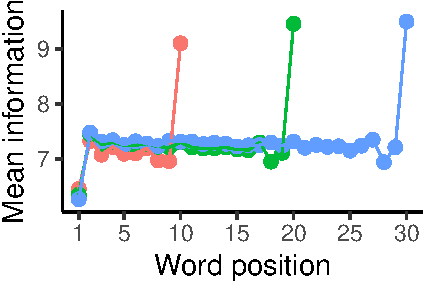
\includegraphics{figs/bnc_unigrams-1.pdf}
\caption{(\#fig:bnc\_unigrams)BNC frequency-based information curves}
\end{figure}

However, this only characterizes written English sentences. If this information distribution is characteristic more generally of English, then we will find the same distribution for spoken English. We use the Switchboard corpus of spoken English telephone conversations between adults to compute the distribution of information across spoken utterances in English. The sentences in the BNC, compared to the conversations in Switchboard, feature much longer sentences with larger vocabularies and more complex sentence structures. We split the conversations in Switchboard not by sentences, as in the BNC, but by turns.

For Switchboard we find the same information trajectory as we did for the BNC, and we find the same distribution of information regardless of utterance length. The longer the utterance, the more pronounced the information distribution shape becomes. A qualitative comparison of the two trajectories is in Figure @ref(fig:switchboard\_unigrams).

\begin{figure}
\centering
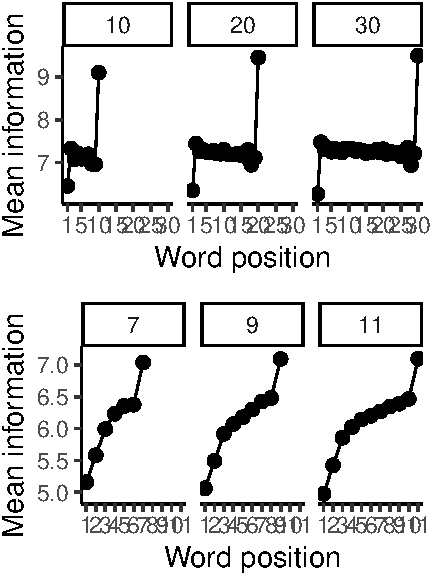
\includegraphics{figs/switchboard_unigrams-1.pdf}
\caption{(\#fig:switchboard\_unigrams)Switchboard frequency-based information curves}
\end{figure}

We have found a unique average distribution of information that appears to characterize the English language as a whole, regardless of medium (spoken or written) or utterance length. This distribution indicates that in English, the words we speak or write at the beginnings of utterances have little information, while the words we speak or write at the ends of utterances have a lot of information. The words in the middle of utterances have a middling amount of information, without the increasing trend in information from word to word that we might expect from (Genzel \& Charniak, 2002).

What about context? So far we've only discussed the frequency-based metric, considering words on their own without any explicit incorporation of prior context. As previously discussed, listeners decode information and process what they hear incrementally, using prior heard words to ease the comprehension process. We now include one word of context (bigrams) and then two words of context (trigrams) for each word in our measurements. We observe a flattening effect of context across both modalities and all speaker populations. After the first word or two, where the listener does not have access to prior context, then they decode information at a flat and more or less uniform rate. The contextual information curves for the BNC and Switchboard are in Figures @ref(fig:switchboard\_bigrams) and @ref(fig:switchboard\_trigrams).

\begin{figure}
\centering
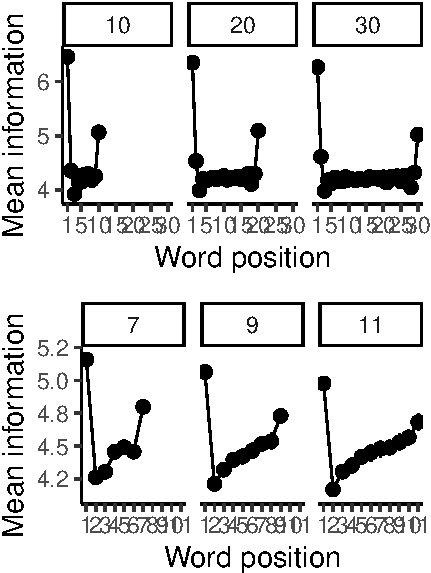
\includegraphics{figs/switchboard_bigrams-1.pdf}
\caption{(\#fig:switchboard\_bigrams)Switchboard bigram context-based information curves}
\end{figure}

\begin{figure}
\centering
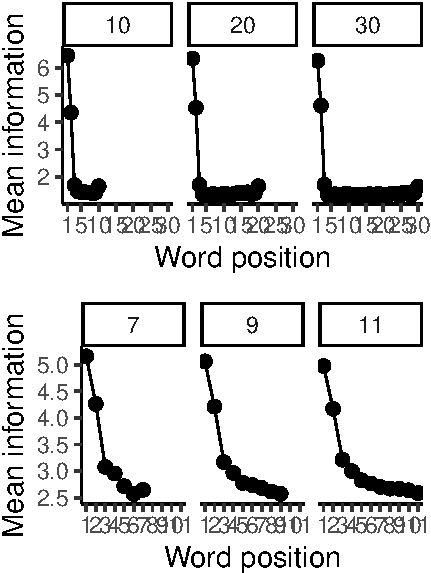
\includegraphics{figs/switchboard_trigrams-1.pdf}
\caption{(\#fig:switchboard\_trigrams)Switchboard trigram context-based information curves}
\end{figure}

Speakers produce information at a more or less constant rate, avoiding peaks or troughs in their information distribution, except at the beginnings of utterances, where listeners may not have any context to predict what the speaker is going to say. Speakers of English tend towards a characteristic and uneven distribution of word information based on frequencies within their utterances. Their interlocutors, however, once they have a word or two of context, decode information at a more or less constant and optimal rate.

\hypertarget{english-cds-and-child-speech}{%
\section{English CDS and child speech}\label{english-cds-and-child-speech}}

We found that English speakers and writers used the same robust and distinctive distribution of information within each utterance, regardless of the number of words in their utterances. To determine if this distribution truly characterizes all speakers of the English language as a whole, we wanted to examine speech from English-speaking children who are producing their very first multi-word utterances. We hypothesize the three-step distribution of information we found for English will characterize child speech and child-directed speech.

We use the Providence corpus from CHILDES (Evans \& Demuth, 2012; MacWhinney, 2000), which consists of about 650000 utterances from parent-child conversations for six monolingual English-speaking children talking with the parents. We obtained the Providence corpus using the childesr frontend to the childes-db database (Sanchez et al., 2019). The child age range was between 11 months and 4 years. Sessions recorded in the home. Parents said a majority of the utterances, but children take up an increasing share of the conversation as they grow older and are actually able to speak full utterances. The utterances in the Providence corpus are on average significantly shorter than those in the BNC and Switchboard; over 90\% of the utterances in the Providence corpus are at most 10 words long, with the median at around 6 words. Similar to our treatment of the Switchboard corpus, we split the Providence corpus up by conversational turns and separate utterances.

We observe the same distinctive distribution of information for parents and children in the Providence corpus as we did for adults in the BNC and Switchboard. The distribution of information we found at the level of individual words in English, therefore, characterizes the English language as a whole and not only adult utterances, not only written utterances. See @ref(fig:providence\_unigrams).

\begin{figure}
\centering
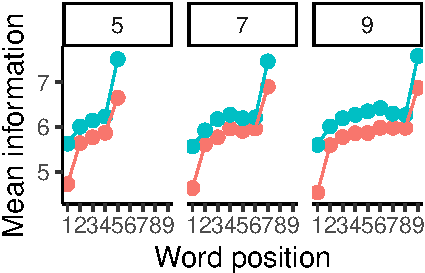
\includegraphics{figs/providence_unigrams-1.pdf}
\caption{(\#fig:providence\_unigrams)Providence frequency-based information curves. Lines around each point indicate 95\% confidence intervals computed with non-parametric bootstrap}
\end{figure}

What about context in the Providence corpus? When incorporating one or two words of predictive context, we observe the same trend as in the Switchboard and BNC corpora. Beyond the first couple of words, once your interlocutor has enough context to predict with some accuracy what you will say next, then you decode information from their speech stream at a constant and optimal rate. This applies to parents and children speaking to one another, as well as adults speaking and writing to one another. See @ref(fig:providence\_bigrams) and @ref(fig:providence\_trigrams).

\begin{figure}
\centering
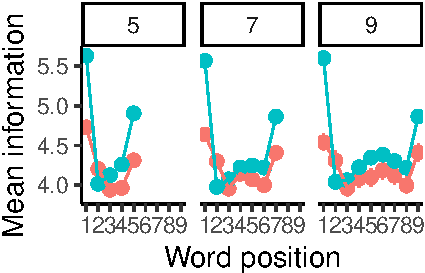
\includegraphics{figs/providence_bigrams-1.pdf}
\caption{(\#fig:providence\_bigrams)Providence bigram context-based information curves}
\end{figure}

\begin{figure}
\centering
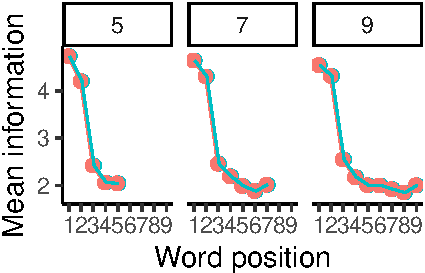
\includegraphics{figs/providence_trigrams-1.pdf}
\caption{(\#fig:providence\_trigrams)Providence trigram context-based information curves}
\end{figure}

\hypertarget{child-speech-and-cds-across-languages}{%
\section{Child speech and CDS across languages}\label{child-speech-and-cds-across-languages}}

So far, we have only looked at the distribution of information in words in English, both with and without context. We have examined child speech, child-directed speech and adult-directed speech, as well as writing samples selected to be representative of British English as a whole. But this only captures the picture for English.

We now turn to a small number of typologically diverse languages, and conduct the same analysis, using a monolingual adult-child speech corpora from CHILDES (MacWhinney, 2000) to compare the results from these languages directly to our results from the English Providence corpus. We use corpora for Spanish, German, French, Mandarin and Japanese. Similarly to the English Providence corpus, all of the following corpora consist mainly of shorter utterances: most utterances in the corpora are under 10 words long. For Spanish, we use the corpus of conversations between primary school-aged children between 6 and 9 years old and the researchers, in which the children were asked to recite stories in their native Spanish (Shiro, 1996). The students came from working class public schools and upper class private schools. For German, we use the Wagner corpus (Wagner, 1985). This corpus consists of a collection of mini-corpora collected from socio-economically diverse families, with children aged from 1;0 to 14;0, mainly on the younger end of that range. The corpus mainly consists of parent-child conversations between the children and their primary caregivers. For French, we use the Palasis corpus (Palasis, 2009), a longitudinal study of children between the ages of 2;5 and 4;0 from the same kindergarten class. The conversations in this corpus take place between the children and other children in the same class, and between the children and the investigator. For Mandarin Chinese, we use the Zhou corpus of dinner conversations from the Shanghai area (Li \& Zhou, 2015). The children in this corpus are 5 or 6 years old, and half come from working class families (the other half from upper class families). For Japanese, we use the Okayama corpus (Shirai, 2001). This corpus consists of conversations between children between the ages of 2;2 and 4;2 and their mothers.

We observe a distinct and characteristic frequency-based information trajectory emerge for each language, robust across each utterance length within each language. We see the same distribution of information for both parents and children in each language, with the child's curve normally below the parent's curve, likely due to the parent speaking a larger share of the utterances in the corpus and using a larger vocabulary than the child. We see the opposite amplitude trend in the Shiro corpus, where the children speak more than the adult investigators as the children are the ones telling the stories. We include the frequency-based information curve from the Providence corpus for comparison.

\begin{figure}
\centering
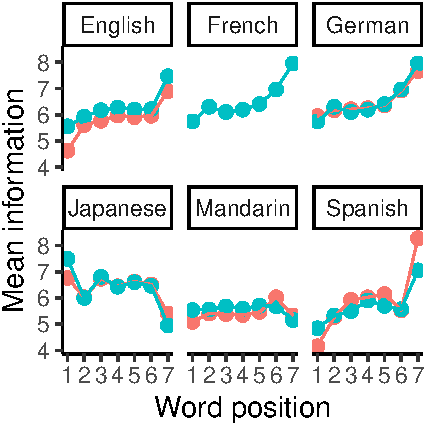
\includegraphics{figs/unnamed-chunk-1-1.pdf}
\caption{\label{fig:unnamed-chunk-1}CHILDES frequency-based information curves}
\end{figure}

English, Spanish, French and German feature similar information curves shapes, with slight variations. The German information curve features lower information for longer towards the beginnings of utterances, possibly due to the grammatical restriction that the second word in German utterances must be a verb (V2). Spanish features a larger spike in the amount of information in the final words of utterances. For Japanese and Mandarin, we observe completely different frequency-based information curve trajectories. The Japanese frequency-based information curve trajectory begins high and finishes low, the mirror image of the European language information curves. The Mandarin curve begins low and finishes low, but features high information in the middle of utterances. We hypothesize this may be due to both Japanese and Mandarin speakers typically ending their utterances with particles, which contain very little information on their own. The penultimate noun with the speakers pair the particles are where the information lies.

For the bigram and trigram information curves, we see the same contextual smoothing effect as for all the corpora we worked with in English. While the frequency-based information curves may depend based on the language, the contextual information curves show the same trajectory cross-linguistically. Using more than two words of context is difficult for parent-child speech corpora because the utterances are so short on average (less than \(10\) words). We hypothesize that the frequency-based information curves may vary based on the genealogy and typology of the languages in question, but this does not extend to the information curves with two words of context in particular.

\begin{figure}
\centering
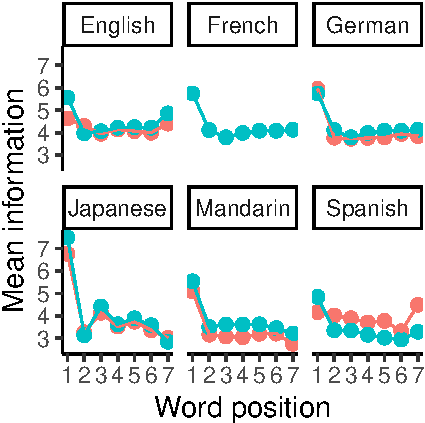
\includegraphics{figs/unnamed-chunk-2-1.pdf}
\caption{\label{fig:unnamed-chunk-2}CHILDES bigram context-based information curves}
\end{figure}

\begin{figure}
\centering
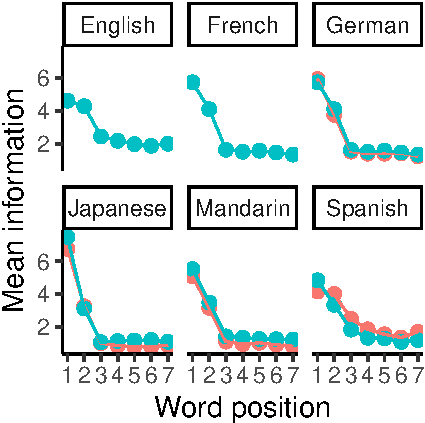
\includegraphics{figs/unnamed-chunk-3-1.pdf}
\caption{\label{fig:unnamed-chunk-3}CHILDES trigram context-based information curves}
\end{figure}

\hypertarget{language-structure-and-large-scale-data-analysis-methods-and-preprocessing}{%
\section{Language structure and large-scale data analysis: methods and preprocessing}\label{language-structure-and-large-scale-data-analysis-methods-and-preprocessing}}

To make a claim about language as a whole and languages on a larger scale, we needed to use larger corpora and a much larger number of languages. We pulled corpora for \(159\) diverse languages from Wikipedia, each of which had at least \(10000\) articles on the knowledge base. We split each article up into sentences; the variance in sentence lengths for Wikipedia was significantly larger than for the CHILDES corpora we used in the previous section. Most sentences in Wikipedia contained between \(10\) and \(30\) words, unlike the CHILDES corpora which mainly contained utterances with under 10 words. We excluded the small fraction of utterances with more than \(50\) words since they were small in number and, from manual inspection, uncharacteristic of typical written sentences.

How do we analyze more than \(40\) different surprisal curves for each language, adding up to several thousand surprisal curves total? We used two different strategies, which yielded identical results upon analysis. Each strategy gave us a five-dimensional vector space embedding for each language in a Wikipedia \enquote{slope space}. For the first strategy, we split each sentence length by number of words into fifths, and computed surprisal values for the closest word position to each quintile. We then computed the slopes between the surprisal values at neighboring quintiles, yielding five slope values for each curve. For the second strategy, we split each sentence length by number of words into sections based on those areas of the surprisal curves that had seemed most important before: between the first and second word; between the second and third word; between the third word and third-to-last word; between the third-to-last word and the second to last word; and between the second-to-last word and the last word. We then similarly computed surprisal values at each of these positions, and similarly computed slopes between the surprisal values at each position, giving us another five slope values for each language summarizing the surprisal curves. Illustrations of these two strategies are in Figure \ref{fig:treatments}

\begin{figure}
\centering
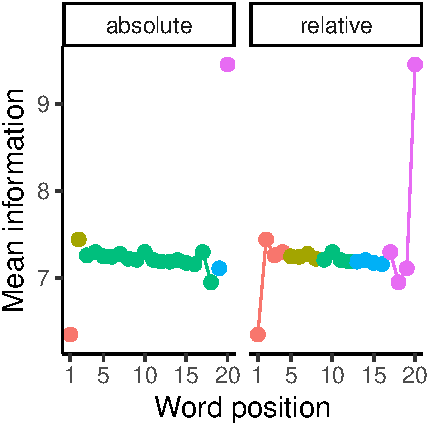
\includegraphics{figs/treatments-1.pdf}
\caption{\label{fig:treatments}Illustration of slope treatments for Wikipedia information curves: relative on top and absolute on bottom}
\end{figure}

We computed unigram, bigram and trigram values for each language, and grouped the contextual and frequency-based values for each treatment.

To more rigorously described the differences between languages, we used data from the World Atlas of Language Structures (WALS; Dryer \& Haspelmath, 2013). WALS has data for \(144\) typological features in \(2569\) languages around the world. These features describe aspects of morphology, syntax, phonology, etymology and semantics--in short the features describe the structures in each language. As WALS is a compiled database from dozens of papers from different authors, most of the features and languages are fairly sparse. Even limiting ourselves to the \(159\) language corpora we pulled from Wikipedia and \(122\) features from WALS, there are nearly \(20000\) individual possible feature values, fewer than half of which were already inputted for those languages in the WALS database.

We used the Multiple Imputation Multiple Correspondence Analysis algorithm (MIMCA; Audigier, Husson, \& Josse, 2017) to fill in the missing data using statistical imputation. MIMCA essentially uses mean imputation to begin with the missing values, then performs repeatedly performs principle components analysis on and reconstructs the contingency table formed from observations in categorical variables. By the end of this we had frequency-based and contextual information curves for the \(159\) language corpora pulled from Wikipedia, along with \(122\) typological features for each language.

However, the WALS features describe specific structural differences between languages, while our surprisal metric is lexical. To target lexical differences between languages, we computed the average normalized Levenshtein distance (LDN; Holman et al., 2008) over the \(40\) item Swadesh list (Swadesh, 1955), retrieved from the ASJP database (Wichmann et al., 2016). The Swadesh list is designed to include near-universal words that target basic cognitive concepts, and are useful in determining the genealogical similarities and differences between languages. The results of classifying languages using the Swadesh list and LDN are correlated with those using WALS features, but the Swadesh list and LDN do not suffer from the same sparsity problem as WALS (Holman et al., 2008).

\hypertarget{language-structures-and-large-scale-data-analysis-results}{%
\section{Language structures and large-scale data analysis: results}\label{language-structures-and-large-scale-data-analysis-results}}

We ran a hierarchical clustering algorithm on the unigram information curves using the hclust package from the R stats core library (Team \& others, 2013). We used the complete linkage algorithm for hierarchical clustering with distances between information curves in language computed using cosine distance between their embeddings in the slope space. The complete linkage algorithm at every step pairs each language or cluster of languages with its closest neighboring language or cluster. A sample from the dendrogram is shown in Figure \ref{fig:dendro}, and the full tree can be constructed using the code in our GitHub repository. The language family-like structure can be seen at first glance, although the dendrogram does not exactly replicate language genealogy for all \(159\) languages. This suggests using a first-pass quantitative method that the information curves do correspond in some measure to language families, but language families do not explain the entire story.

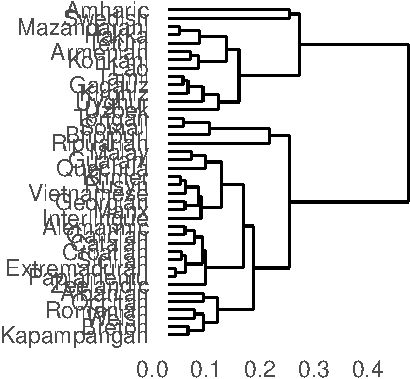
\includegraphics{figs/dendro-1.pdf}

A sample of the contextual information curves (two words of context) are plotted in Figure @ref(fig:wiki\_trigrams), and all trigram information curves for the languages we used follow the same pattern. The first few words in utterances for each language are surprising, but with even a couple words of predictive context for each word, the amount of information in each word drops off and speakers produce information at a constant, optimal rate.

\begin{figure}
\centering
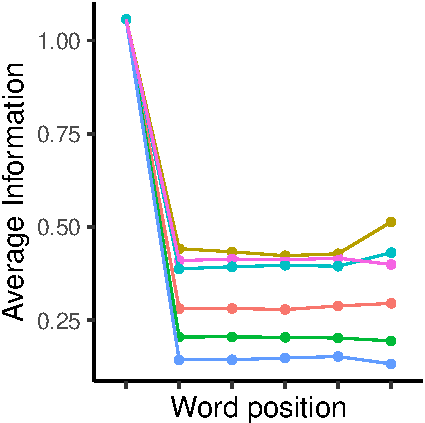
\includegraphics{figs/wiki_trigrams-1.pdf}
\caption{(\#fig:wiki\_trigrams)Some trigram information curves from the Wikipedia data}
\end{figure}

First we examined the effects of individual typological features on the shapes of the unigram information curves. We ran logistic regressions using the lme4 package in R (Bates, Mächler, Bolker, \& Walker, 2014), checking whether the cosine distance between two languages' embeddings in the slope space played a role in determining if they had the same value for a given WALS feature. Individual WALS features do not necessarily have ordinal values. Some, such as the \enquote{Number of Cases} feature, are easy to quantify and order. Others are more difficult. For example, how does one order \enquote{relative clauses appear after the nouns they modify}, \enquote{relative clauses appear before the nouns they modify} and \enquote{free order of relative clauses and nouns}? We chose the identify relation to avoid deciding on the basis of individual features. We found that 100 out of the 120 features from WALS we examined was statistically significant (p \textless{} .001) in determining whether two languages had the same shape to their unigram information distributions. The results for some important features are in Figure @ref(fig:linear\_models), and the rest of the results are in the Appendices.

\begin{figure}
\centering
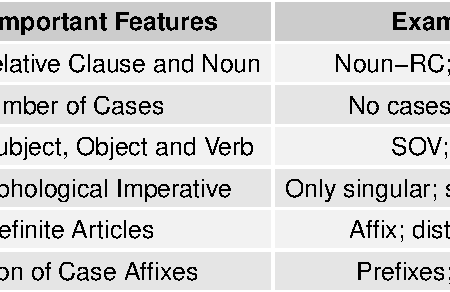
\includegraphics{figs/linear_models-1.pdf}
\caption{(\#fig:linear\_models)Some linear model results from Wikipedia and WALS features}
\end{figure}

We next compared how the cosine distance between two languages related to how many WALS features they had in common. \(r^2\) value is \(.005734\), which suggests that in aggregate there is not a correlation between how many WALS features languages have in common and the similarity of their frequency-based information curves. Figure @ref(fig:cosine\_wals) displays the results. This result is surprising based on the significance of many WALS features in predicting the shapes of the frequency-based information curves, and we return to this result in the general discussion.

\begin{figure}
\centering
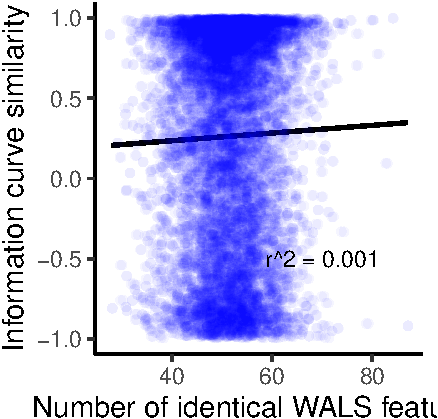
\includegraphics{figs/cosine_wals-1.pdf}
\caption{(\#fig:cosine\_wals)wals features vs cosine similarity}
\end{figure}

For lexical features, we see a stronger correlation between the similarity of two languages in terms of their average LDN and the cosine distance between their information curves. Figure @ref(fig:cosine\_ldn). We see a higher \(r^2\) value here of \(.026\), indicating that there is more correspondence between a language's lexical similarity to another language and their similarity in information curves.

\begin{figure}
\centering
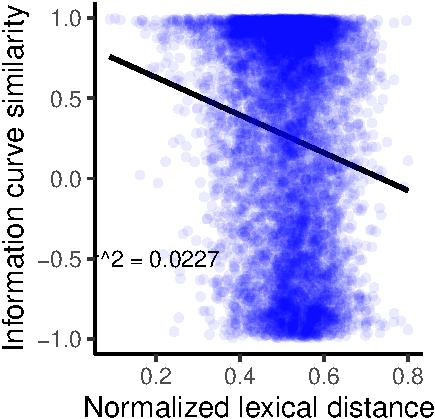
\includegraphics{figs/cosine_ldn-1.pdf}
\caption{(\#fig:cosine\_ldn)ldn features vs cosine similarity}
\end{figure}

From these typological investigations, we conclude that the shape of a language's frequency-based information curve covaries with its typological and lexical similarity to other languages.

\hypertarget{discussion}{%
\section{Discussion}\label{discussion}}

By considering the distribution of information at the level of utterances and sentences, we join together the information-theoretic work focusing on sub-word units and words, and that focusing on paragraphs. In doing so, we show that frequency and context-based metrics complement one another in studying efficiency and information in language. We directly link linguistic efficiency in a language to the genealogy and properties of that language, We provide evidence for a novel linguistic universal: low processing cost for listeners beyond the first words in utterances, driven by high average word predictability in conversation. Also considering the developmental angle, observing language-specific information distributions arising as soon as children begin speaking in multi-word utterances.

Throughout this work we have averaged the surprisal values at each position. Averaging removes variation, which in turn may obscure trends in the data. As discussed in the methods section, the surprisal metric has historically been used for calculating the information and processing cost for individual utterances, and our use of the metric here is actually a step forward rather than a step back. Future work can investigate variation in how speakers distribute information in individual utterances.

The WALS database we used to investigate typological variation in the information curves is overall sparse. We imputed well over \(50\%\) of the WALS features for most of our \(159\) languages, although all of the languages had at least \(20\) features evaluated in WALS. A large part of this is due to WALS being a collection of a number of different studies, instead of a systematic effort to catalogue variation across the world's languages. Additionally, WALS features are meant to describe specific microvariations in languages, not to provide a comprehensive typological representation of each language compared to each other language. This may be why the Swadesh list provided a higher correlation for describing the differences in information curves: Swadesh (1955) intended the list to allow researchers to more comprehensively compared and constrast lexical differences between languages. For our Wikipedia analysis, we also reduce all of a language's variation down to a five-dimensional vector. These information curve representations show a surprising amount of variation despite the degree of compression.

\newpage

\hypertarget{references}{%
\section{References}\label{references}}

\begingroup
\setlength{\parindent}{-0.5in}
\setlength{\leftskip}{0.5in}

\hypertarget{refs}{}
\leavevmode\hypertarget{ref-anderson1989}{}%
Anderson, J. R., \& Milson, R. (1989). Human memory: An adaptive perspective. \emph{Psychological Review}, \emph{96}(4), 703.

\leavevmode\hypertarget{ref-audigier2017}{}%
Audigier, V., Husson, F., \& Josse, J. (2017). MIMCA: Multiple imputation for categorical variables with multiple correspondence analysis. \emph{Statistics and Computing}, \emph{27}(2), 501--518.

\leavevmode\hypertarget{ref-austin1975}{}%
Austin, J. L. (1975). \emph{How to do things with words}. Oxford university press.

\leavevmode\hypertarget{ref-aylett2004}{}%
Aylett, M., \& Turk, A. (2004). The smooth signal redundancy hypothesis: A functional explanation for relationships between redundancy, prosodic prominence, and duration in spontaneous speech. \emph{Language and Speech}, \emph{47}(1), 31--56.

\leavevmode\hypertarget{ref-bates2014}{}%
Bates, D., Mächler, M., Bolker, B., \& Walker, S. (2014). Fitting linear mixed-effects models using lme4. \emph{arXiv Preprint arXiv:1406.5823}.

\leavevmode\hypertarget{ref-chen1999empirical}{}%
Chen, S. F., \& Goodman, J. (1999). An empirical study of smoothing techniques for language modeling. \emph{Computer Speech \& Language}, \emph{13}(4), 359--394.

\leavevmode\hypertarget{ref-wals}{}%
Dryer, M. S., \& Haspelmath, M. (Eds.). (2013). \emph{WALS online}. Leipzig: Max Planck Institute for Evolutionary Anthropology. Retrieved from \url{https://wals.info/}

\leavevmode\hypertarget{ref-evans2012}{}%
Evans, K. E., \& Demuth, K. (2012). Individual differences in pronoun reversal: Evidence from two longitudinal case studies. \emph{Journal of Child Language}, \emph{39}(1), 162--191.

\leavevmode\hypertarget{ref-frank2008}{}%
Frank, A. F., \& Jaeger, T. F. (2008). Speaking rationally: Uniform information density as an optimal strategy for language production. In \emph{Proceedings of the annual meeting of the cognitive science society} (Vol. 30).

\leavevmode\hypertarget{ref-frank2015}{}%
Frank, S. L., Otten, L. J., Galli, G., \& Vigliocco, G. (2015). The erp response to the amount of information conveyed by words in sentences. \emph{Brain and Language}, \emph{140}, 1--11.

\leavevmode\hypertarget{ref-genzel2002}{}%
Genzel, D., \& Charniak, E. (2002). Entropy rate constancy in text. In \emph{Proceedings of the 40th annual meeting of the association for computational linguistics} (pp. 199--206).

\leavevmode\hypertarget{ref-heafield2013scalable}{}%
Heafield, K., Pouzyrevsky, I., Clark, J. H., \& Koehn, P. (2013). Scalable modified kneser-ney language model estimation. In \emph{Proceedings of the 51st annual meeting of the association for computational linguistics (volume 2: Short papers)} (pp. 690--696).

\leavevmode\hypertarget{ref-holman2008}{}%
Holman, E. W., Wichmann, S., Brown, C. H., Velupillai, V., Müller, A., Bakker, D., \& others. (2008). Advances in automated language classification. \emph{Quantitative Investigations in Theoretical Linguistics}, 40--43.

\leavevmode\hypertarget{ref-jaeger2007}{}%
Jaeger, T. F., \& Levy, R. P. (2007). Speakers optimize information density through syntactic reduction. In \emph{Advances in neural information processing systems} (pp. 849--856).

\leavevmode\hypertarget{ref-kemp2012kinship}{}%
Kemp, C., \& Regier, T. (2012). Kinship categories across languages reflect general communicative principles. \emph{Science}, \emph{336}(6084), 1049--1054.

\leavevmode\hypertarget{ref-kirby2015compression}{}%
Kirby, S., Tamariz, M., Cornish, H., \& Smith, K. (2015). Compression and communication in the cultural evolution of linguistic structure. \emph{Cognition}, \emph{141}, 87--102.

\leavevmode\hypertarget{ref-kutas2011}{}%
Kutas, M., \& Federmeier, K. D. (2011). Thirty years and counting: Finding meaning in the n400 component of the event-related brain potential (erp). \emph{Annual Review of Psychology}, \emph{62}, 621--647.

\leavevmode\hypertarget{ref-leech1992}{}%
Leech, G. N. (1992). 100 million words of english: The british national corpus (bnc).

\leavevmode\hypertarget{ref-levy2008}{}%
Levy, R. (2008). Expectation-based syntactic comprehension. \emph{Cognition}, \emph{106}(3), 1126--1177.

\leavevmode\hypertarget{ref-li2015}{}%
Li, H., \& Zhou, J. (2015). \emph{Study on dinner table talk of preschool children family in shanghai} (Master's thesis). East China Normal University, Shanghai, China.

\leavevmode\hypertarget{ref-macwhinney2000}{}%
MacWhinney, B. (2000). \emph{The childes project: The database} (Vol. 2). Psychology Press.

\leavevmode\hypertarget{ref-mahowald2013}{}%
Mahowald, K., Fedorenko, E., Piantadosi, S. T., \& Gibson, E. (2013). Info/information theory: Speakers choose shorter words in predictive contexts. \emph{Cognition}, \emph{126}(2), 313--318.

\leavevmode\hypertarget{ref-palasis2009}{}%
Palasis, K. (2009). \emph{Syntaxe générative et acquisition: Le sujet dans le développement du système linguistique du jeune enfant} (PhD thesis). Nice.

\leavevmode\hypertarget{ref-perfors2014language}{}%
Perfors, A., \& Navarro, D. J. (2014). Language evolution can be shaped by the structure of the world. \emph{Cognitive Science}, \emph{38}(4), 775--793.

\leavevmode\hypertarget{ref-piantadosi2011}{}%
Piantadosi, S. T., Tily, H., \& Gibson, E. (2011). Word lengths are optimized for efficient communication. \emph{Proceedings of the National Academy of Sciences}, \emph{108}(9), 3526--3529.

\leavevmode\hypertarget{ref-pickering2013}{}%
Pickering, M. J., \& Garrod, S. (2013). An integrated theory of language production and comprehension. \emph{Behavioral and Brain Sciences}, \emph{36}(4), 329--347.

\leavevmode\hypertarget{ref-sanchez2019}{}%
Sanchez, A., Meylan, S. C., Braginsky, M., MacDonald, K. E., Yurovsky, D., \& Frank, M. C. (2019). Childes-db: A flexible and reproducible interface to the child language data exchange system. \emph{Behavior Research Methods}, \emph{51}(4), 1928--1941.

\leavevmode\hypertarget{ref-shannon1948}{}%
Shannon, C. E. (1948). A mathematical theory of communication. \emph{Bell System Technical Journal}, \emph{27}(3), 379--423.

\leavevmode\hypertarget{ref-shirai2001}{}%
Shirai, Y. (2001). The acquisition of causative morphology in japanese: A prototype account. \emph{East Asian Language Acquisition}.

\leavevmode\hypertarget{ref-shiro1996}{}%
Shiro, M. L. de. (1996). Un estudio de las expresiones de modalidad en hablantes de dos culturas. \emph{Boletı'n de Lingüı'stica}, (10), 43--60.

\leavevmode\hypertarget{ref-smith2013}{}%
Smith, N. J., \& Levy, R. (2013). The effect of word predictability on reading time is logarithmic. \emph{Cognition}, \emph{128}(3), 302--319.

\leavevmode\hypertarget{ref-swadesh1955}{}%
Swadesh, M. (1955). Towards greater accuracy in lexicostatistic dating. \emph{International Journal of American Linguistics}, \emph{21}(2), 121--137.

\leavevmode\hypertarget{ref-tanenhaus1995}{}%
Tanenhaus, M. K., Spivey-Knowlton, M. J., Eberhard, K. M., \& Sedivy, J. C. (1995). Integration of visual and linguistic information in spoken language comprehension. \emph{Science}, \emph{268}(5217), 1632--1634.

\leavevmode\hypertarget{ref-team2013}{}%
Team, R. C., \& others. (2013). R: A language and environment for statistical computing.

\leavevmode\hypertarget{ref-wagner1985}{}%
Wagner, K. R. (1985). How much do children say in a day? \emph{Journal of Child Language}, \emph{12}(2), 475--487.

\leavevmode\hypertarget{ref-wichmann2016}{}%
Wichmann, S., Müller, A., Wett, A., Velupillai, V., Bischoffberger, J., Brown, C. H., \ldots{} others. (2016). The asjp database. \emph{Max Planck Institute for the Science of Human History, Jena}.

\leavevmode\hypertarget{ref-yu2016}{}%
Yu, S., Cong, J., Liang, J., \& Liu, H. (2016). The distribution of information content in english sentences. \emph{arXiv Preprint arXiv:1609.07681}.

\endgroup


\end{document}
